\chapter{Numerical Platform}

\section{Overview} 

\begin{figure}[h!]
\centering
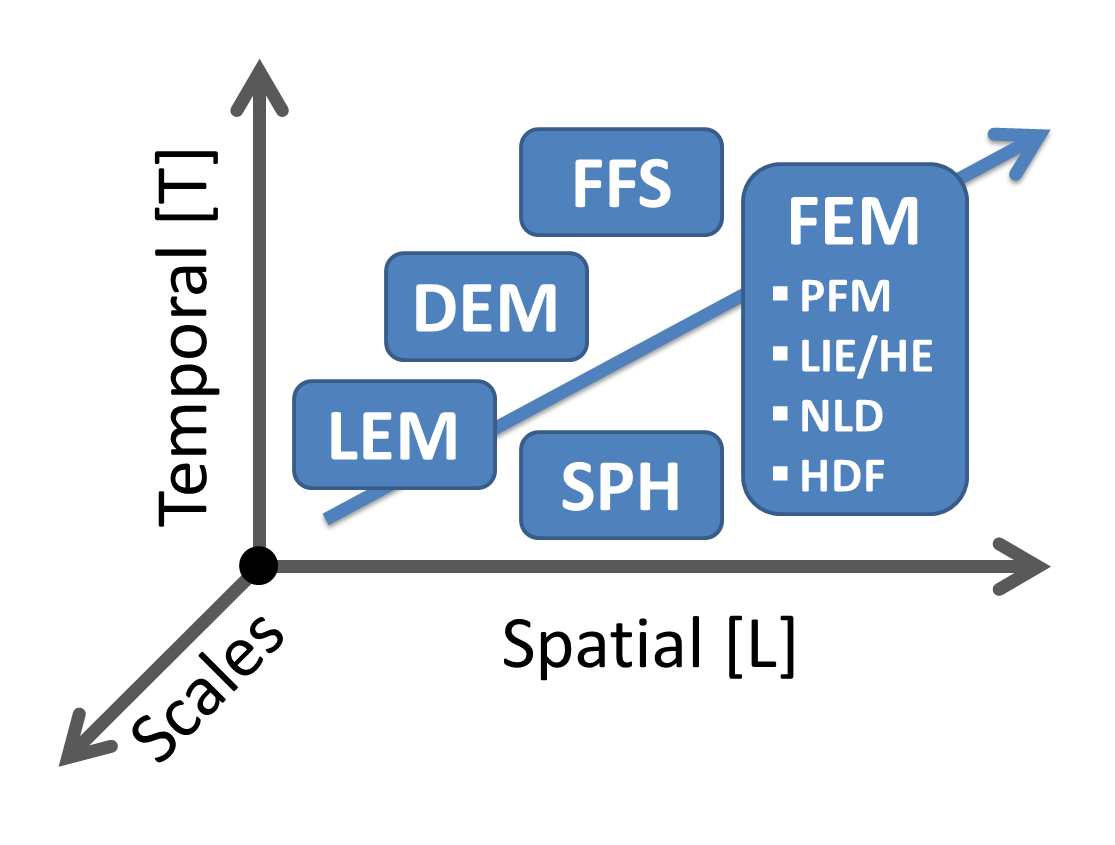
\includegraphics[width=1\textwidth]{figures/geomint-mod-overview}
\label{fig:20}
\caption{}
\end{figure}

\section{Numerical Methods}
2-3 pages brief introduction per method (ca. 25)
\subsection{FFS - Forces on Fracture Surfaces}
\subsection{LEM - Lattice-Element-Method}
\subsection{DEM - Distinct-Element-Method}
\subsection{SPH - Smoothed-Particle-Hydrodynamics}
\subsection{FEM - Finite-Element-Method}
\subsubsection{LIE - Lower-Interface-Elements}
\subsubsection{HDF - Hybrid-Dimensional-Formulation}
\subsubsection{PFM - Variational Phase-Field Method}
\subsubsection{NLD - Non-Local Dynamics}
